\documentclass[crop,tikz]{standalone}
\usepackage{tikz}
\usetikzlibrary{matrix,backgrounds,arrows.meta,fit,positioning,decorations.pathreplacing}
\begin{document}

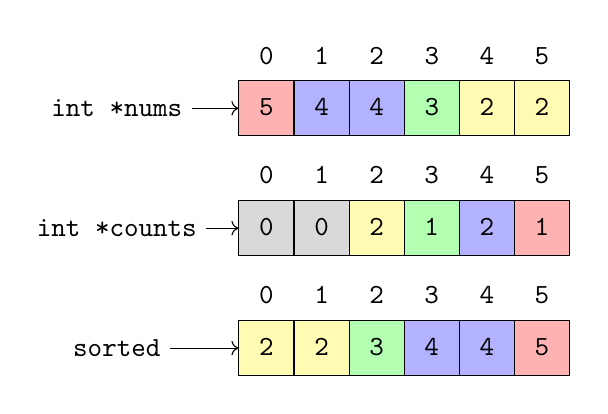
\begin{tikzpicture}[font=\ttfamily,
  array/.style={matrix of nodes,nodes={draw, fill=green!30,minimum size=7mm},column sep=-\pgflinewidth, row sep=0.5mm, nodes in empty cells,text height=1.5ex, text depth=.25ex,
    row 1/.style={nodes={draw=none, fill=none, minimum size=5mm}},
    row 2 column 5/.style={nodes={fill=yellow!30}},
    row 2 column 6/.style={nodes={fill=yellow!30}},
    row 2 column 2/.style={nodes={fill=blue!30}},
    row 2 column 3/.style={nodes={fill=blue!30}},
    row 2 column 1/.style={nodes={fill=red!30}},
  },
  counts/.style={
    row 2 column 1/.style={nodes={fill=gray!30}},
    row 2 column 2/.style={nodes={fill=gray!30}},
    row 2 column 3/.style={nodes={fill=yellow!30}},
    row 2 column 5/.style={nodes={fill=blue!30}},
    row 2 column 6/.style={nodes={fill=red!30}},
  },
  sorted/.style={
    row 2 column 1/.style={nodes={fill=yellow!30}},
    row 2 column 2/.style={nodes={fill=yellow!30}},
    row 2 column 3/.style={nodes={fill=green!30}},
    row 2 column 4/.style={nodes={fill=blue!30}},
    row 2 column 5/.style={nodes={fill=blue!30}},
    row 2 column 6/.style={nodes={fill=red!30}},
  },
]

\matrix[array] (array) {
 0 & 1 & 2 & 3 & 4 & 5 \\
  5 & 4 & 4 & 3 & 2 & 2 \\ };

\matrix[array,counts,below=0.01cm of array] (counts) {
 0 & 1 & 2 & 3 & 4 & 5 \\
  0 & 0 & 2 & 1 & 2 & 1 \\ };

\matrix[array,sorted,below=0.01cm of counts] (sorted) {
 0 & 1 & 2 & 3 & 4 & 5 \\
  2 & 2 & 3 & 4 & 4 & 5 \\ };

\draw[->] node[left of=array-2-1,xshift=-9mm] {int *nums} edge (array-2-1);
\draw[->] node[left of=counts-2-1,xshift=-9mm] {int *counts} edge (counts-2-1);
\draw[->] node[left of=sorted-2-1,xshift=-9mm] {sorted} edge (sorted-2-1);

\end{tikzpicture}
\end{document}
